\documentclass[tikz,border=4pt]{standalone}
\usepackage[utf8]{inputenc}
\usepackage[T1]{fontenc}
\usepackage{amsmath}
\usepackage{pgfplots}
\usepgfplotslibrary{groupplots}
\pgfplotsset{compat=1.18}
\begin{document}
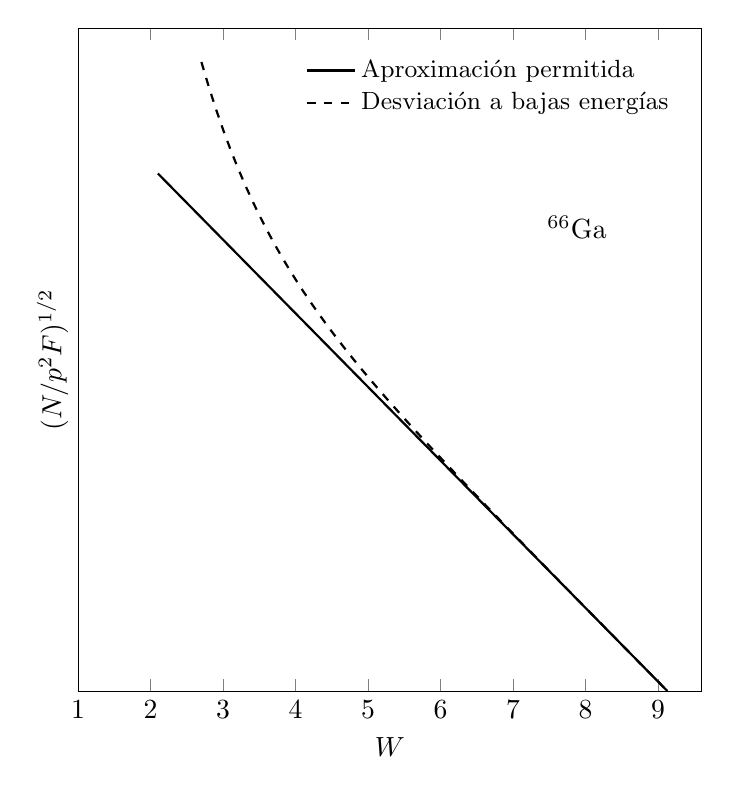
\begin{tikzpicture}
\begin{axis}[width=9.5cm, height=10cm, xmin=1, xmax=9.6, ymin=0, ymax=9,
  xtick={1,2,...,9}, ytick=\empty, xlabel={$W$}, ylabel={$(N/p^2F)^{1/2}$},
  legend style={at={(0.97,0.97)}, anchor=north east, font=\small, draw=none, fill=none},
  legend cell align=left]
\addplot[thick] coordinates {(2.1,7.0272) (9.1272,0)};
\addplot[thick, dashed] coordinates {(2.7,8.5407) (2.8,8.2098) (2.9,7.9037) (3,7.6198) (3.1,7.3557) (3.2,7.1094) (3.3,6.8788) (3.4,6.6624) (3.5,6.4586) (3.6,6.2661) (3.7,6.0837) (3.8,5.9103) (3.9,5.7449) (4,5.5867) (4.1,5.4349) (4.2,5.2887) (4.3,5.1477) (4.4,5.0112) (4.5,4.8787) (4.6,4.7499) (4.7,4.6242) (4.8,4.5014) (4.9,4.3812) (5,4.2633) (5.1,4.1473) (5.2,4.0332) (5.3,3.9207) (5.4,3.8096) (5.5,3.6997) (5.6,3.591) (5.7,3.4833) (5.8,3.3765) (5.9,3.2705) (6,3.1651) (6.1,3.0604) (6.2,2.9563) (6.3,2.8526) (6.4,2.7494) (6.5,2.6465) (6.6,2.544) (6.7,2.4418) (6.8,2.3399) (6.9,2.2382) (7,2.1367) (7.1,2.0354) (7.2,1.9342) (7.3,1.8332) (7.4,1.7324) (7.5,1.6316) (7.6,1.5309) (7.7,1.4304) (7.8,1.3299) (7.9,1.2294) (8,1.1291) (8.1,1.0287) (8.2,0.92845) (8.3,0.82821) (8.4,0.728) (8.5,0.62783) (8.6,0.52768) (8.7,0.42755) (8.8,0.32744) (8.9,0.22735) (9,0.12728) (9.1,0.027216) (9.1272,0)};
\legend{Aproximaci\'on permitida, Desviaci\'on a bajas energ\'ias}
\node at (rel axis cs:0.80,0.70) {$^{66}$Ga};
\end{axis}
\end{tikzpicture}
\end{document}
